\subsection{Q15 Format} \label{sec:q15}

For our filter design, fixed format number format called Q is used. Unlike floating point numbers, Q-format numbers require only a standard integer Arithmetic Logic Unit (ALU) to perform rational number calculations. This means that we do not need to add an Floating Point Unit (FPU) to our design, which requires additional power.

Q format numbers are represented using the Q notation which is written as Q$m,n$ where $m$ is the number of bits set aside to designate the two's complement integer portion of the number, and $n$ is the number of bits used to designate the fractional portion of the number.

In our case, we use simplified notation Q$n$ since we assume that the numbers are normalized into the range of $[-1, 1)$. Notice that this assumption does not affect the generality of the filter, but it simplifies the multiplication operation because the multiplication result never exceeds the range of $[-1, 1)$.

\begin{figure}[htbp]
	\centering
	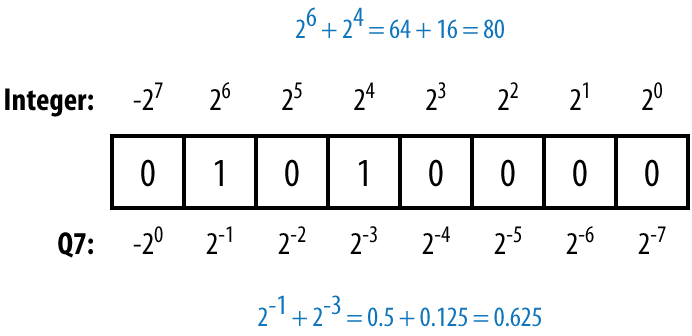
\includegraphics[scale=1.5]{images/q7}
	\caption{Comparison between integer and Q7 format.}
	\label{fig:q7}
\end{figure}

Figure \ref{fig:q7} shows the comparison between two's complement integer and Q7 numbers. The only difference between the two is the weight assigned for each bit.

\subsection{Filter Characteristics}

\begin{table}[htbp]
\centering
\begin{tabular}{ c | r | r }
\hline
Coeffiecient & Value & Q15 \\
\hline \hline
$C_0$ & -0.022663985459552   & \texttt{1111110100011010} \\
$C_1$ & 1.04697822237622e-17 & \texttt{0000000000000000} \\
$C_2$ & 0.273977082565524    & \texttt{0010001100010001}\\
$C_3$ & 0.497373805788057    & \texttt{0011111110101001}\\
$C_4$ & 0.273977082565524    & \texttt{0010001100010001}\\
$C_5$ & 1.04697822237622e-17 & \texttt{0000000000000000} \\
$C_6$ & -0.022663985459552   & \texttt{1111110100011010} \\
\end{tabular}
\caption{Coefficient values.}
\label{tab:coefficients}
\end{table}

The coefficients for the filter is shown in Table \ref{tab:coefficients}. These values were computed using Filter Design \& Analysis Tool (Figure \ref{fig:matlab}) in Matlab Signal Processing Toolbox which is one of the most widely used filter design tools in the industry. We have chosen a $8^{\rm th}$ order FIR filter with a Hamming window. This filter is also one of the most widely used in the industry and has straight-forward characteristic.

\begin{figure}[htbp]
	\centering
	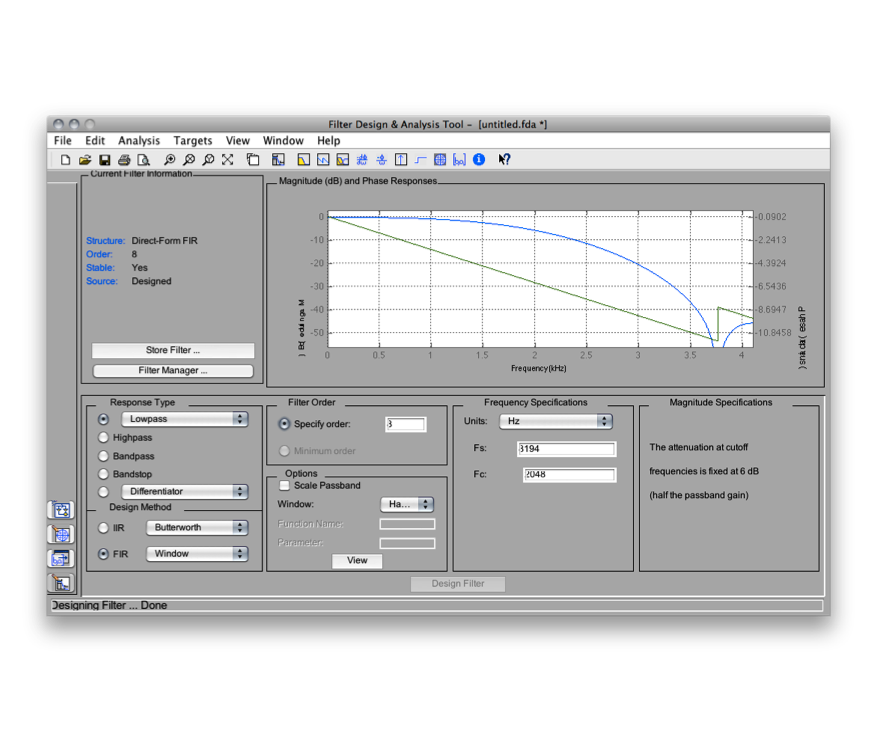
\includegraphics[width=6.5in]{images/matlab}
	\caption{Matlab Filter Design \& Analysis Tool.}
	\label{fig:matlab}
\end{figure}
